\documentclass[slovene]{beamer}
\usepackage[utf8]{inputenc}
\usepackage{amsmath}
\usepackage{graphicx}
\usepackage{booktabs}
\usepackage{babel}
\usepackage{hyperref}

\title{Optična rotacija raztopine saharoze}
\author{Matija Zanjkovič, Mesarec Tilen, Petauer Maja}
\date{Junij 2025}

\begin{document}

\begin{frame}
    \titlepage
\end{frame}

\begin{frame}{Uvod}
    \begin{itemize}
        \item Raziskovali smo optično rotacijo polarizirane svetlobe.
        \item Kaj je optična rotacija in zakaj se pojavi?
        \item Enantiomeri: zrcalne slike, ki se ne prekrivajo.
    \end{itemize}
    \begin{center}
        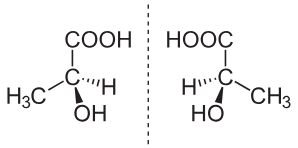
\includegraphics[width=0.5\textwidth]{slike/enantiomer.png}
    \end{center}
\end{frame}

\begin{frame}{Kiralnost in optična aktivnost}
    \begin{itemize}
        \item Voda ni enantiomer (simetrična).
        \item Sladkorji (glukoza, fruktoza, saharoza) so kiralni.
        \item Kiralnost: različne lastnosti v kiralnem okolju.
        \item Optična rotacija: enantiomeri rotirajo polarizirano svetlobo v nasprotni smeri.
    \end{itemize}
    \begin{center}
        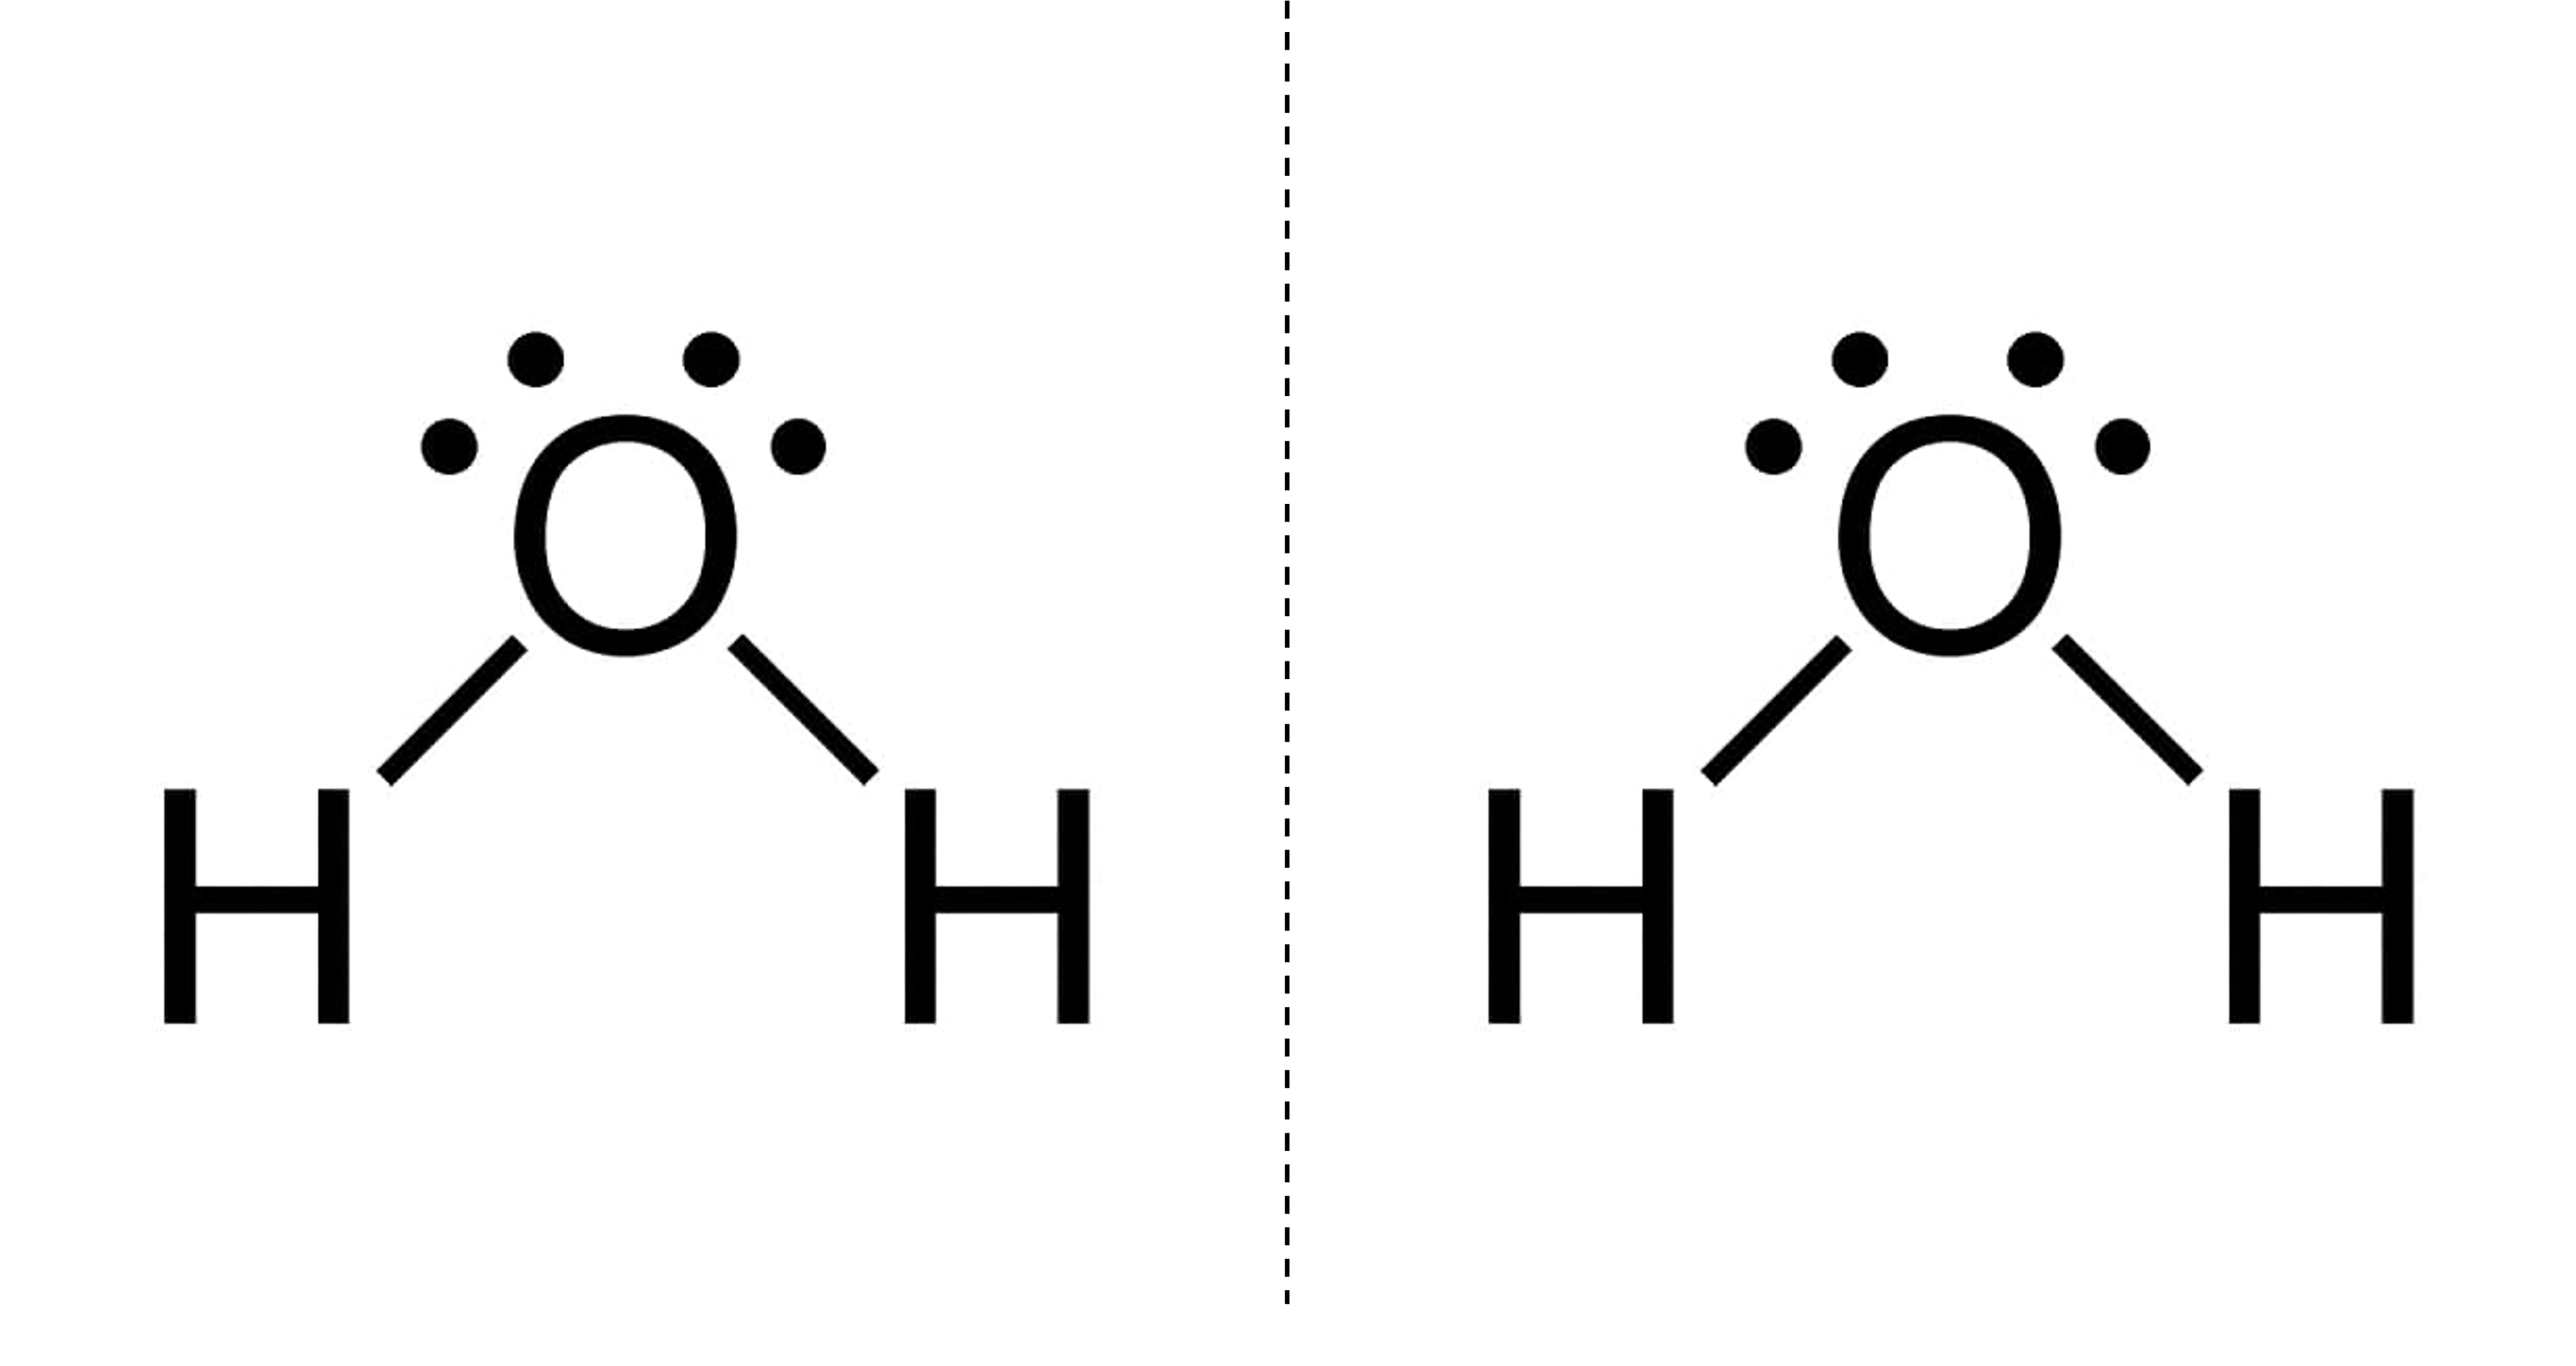
\includegraphics[width=0.5\textwidth]{slike/voda.png}
    \end{center}
\end{frame}

\begin{frame}{Cilji in teorija}
    \begin{itemize}
        \item Izmeriti specifično rotacijo saharoze v vodi pri različnih koncentracijah in dveh valovnih dolžinah (rdeča, zelena).
        \item Preveriti Drudejev model disperzije.
    \end{itemize}
    \[
        [\alpha]^{\text{T}}_{\lambda}= \frac{\alpha}{c \cdot l}
    \]
    \[
        \left[ [\alpha] \right] = \left[ \frac{^\circ \cdot \mathrm{dm}}{\mathrm{g} \cdot \mathrm{mL}} \right]
    \]
\end{frame}

\begin{frame}{Eksperimentalna izvedba}
    \begin{itemize}
        \item Priprava raztopin saharoze različnih koncentracij.
        \item Merjenje kota rotacije z laserjem (rdeča in zelena).
        \item Uporaba polarizatorjev in LoggerPro.
    \end{itemize}
    \begin{center}
        \includegraphics[width=0.5\textwidth]{slike/setup.png}
    \end{center}
\end{frame}

\begin{frame}{Merjene količine}
    \begin{itemize}
        \item Koncentracija saharoze $c$ (g/mL)
        \item Valovna dolžina $\lambda$ (nm)
        \item Kot rotacije $\alpha$ (°)
        \item Dolžina cevi $l$ (dm)
    \end{itemize}
\end{frame}

\begin{frame}{Primer rezultatov -- meritve}
    \begin{table}[ht]
    \centering
    \begin{tabular}{cccc}
    \toprule
    $c$ [g/mL] & $\alpha_r$ [°] & $\alpha_z$ [°] & $\Delta\alpha$ [°] \\
    \midrule
    0.000 & 75  & 79  & 2 \\
    0.030 & 90  & 96  & 2 \\
    0.050 & 102 & 110 & 2 \\
    0.070 & 115 & 126 & 2 \\
    0.090 & 131 & 136 & 2 \\
    0.100 & 137 & 141 & 2 \\
    \bottomrule
    \end{tabular}
    \end{table}
\end{frame}

\begin{frame}{Izračun specifične rotacije}
    \[
        [\alpha] = \frac{\alpha}{c \cdot L}
    \]
    \begin{itemize}
        \item Primer za rdečo:
        \item $[\alpha]_{c=0.030} = 43 \ (1 \pm 0.36)$
        \item $[\alpha]_{c=0.100} = 54 \ (1 \pm 0.14)$
    \end{itemize}
    \begin{itemize}
        \item Primer za zeleno:
        \item $[\alpha]_{c=0.030} = 49 \ (1 \pm 0.33)$
        \item $[\alpha]_{c=0.100} = 56 \ (1 \pm 0.14)$
    \end{itemize}
\end{frame}

\begin{frame}{Povprečna specifična rotacija}
    \[
    \overline{[\alpha]}_{\text{rdeča}} = 50
    \]
    \[
    \overline{[\alpha]}_{\text{zelena}} = 54
    \]
\end{frame}

\begin{frame}{Med -- analiza}
    \begin{itemize}
        \item Naravni med: glukoza in fruktoza ($36:41$)
        \item $[\alpha]_{glukoza} = 53$, $[\alpha]_{fruktoza} = -92$
        \item $[\alpha]_{med} = -24$
        \item Sintetični med: $7 - 89$
    \end{itemize}
    \begin{center}
        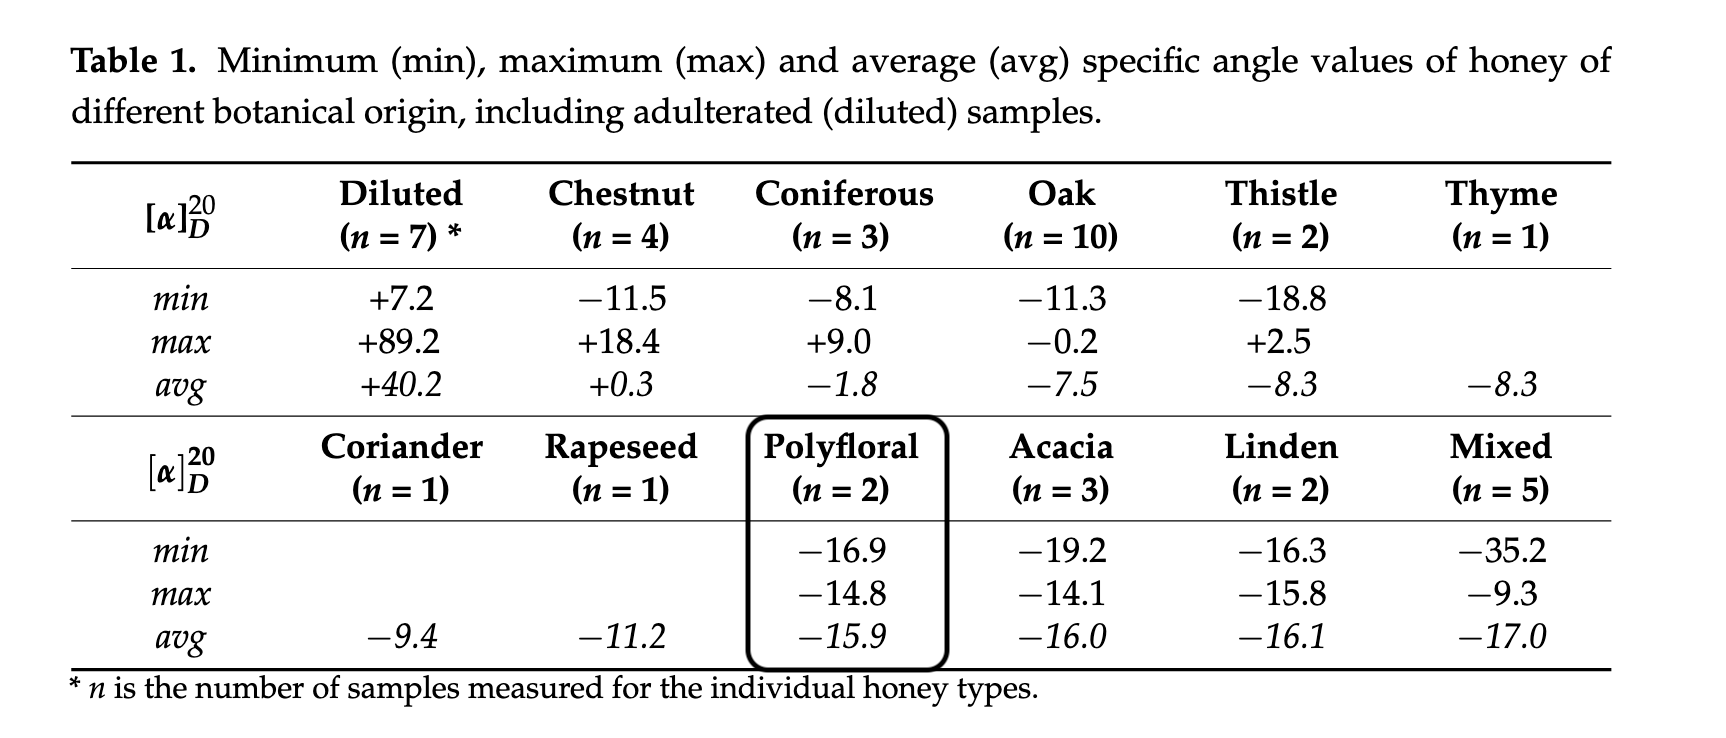
\includegraphics[width=0.7\textwidth]{slike/med.png}
    \end{center}
\end{frame}

\begin{frame}{Rezultati za med}
    \begin{itemize}
        \item Prvi med: $[\alpha]_{med_1} = -70 \pm 87$
        \item Drugi med: $[\alpha]_{med_2} = 52 \pm 65$
        \item Velike napake zaradi majhnega kota in koncentracije.
        \item Med$_1$ kristaliziral, med$_2$ ni.
    \end{itemize}
    \begin{center}
        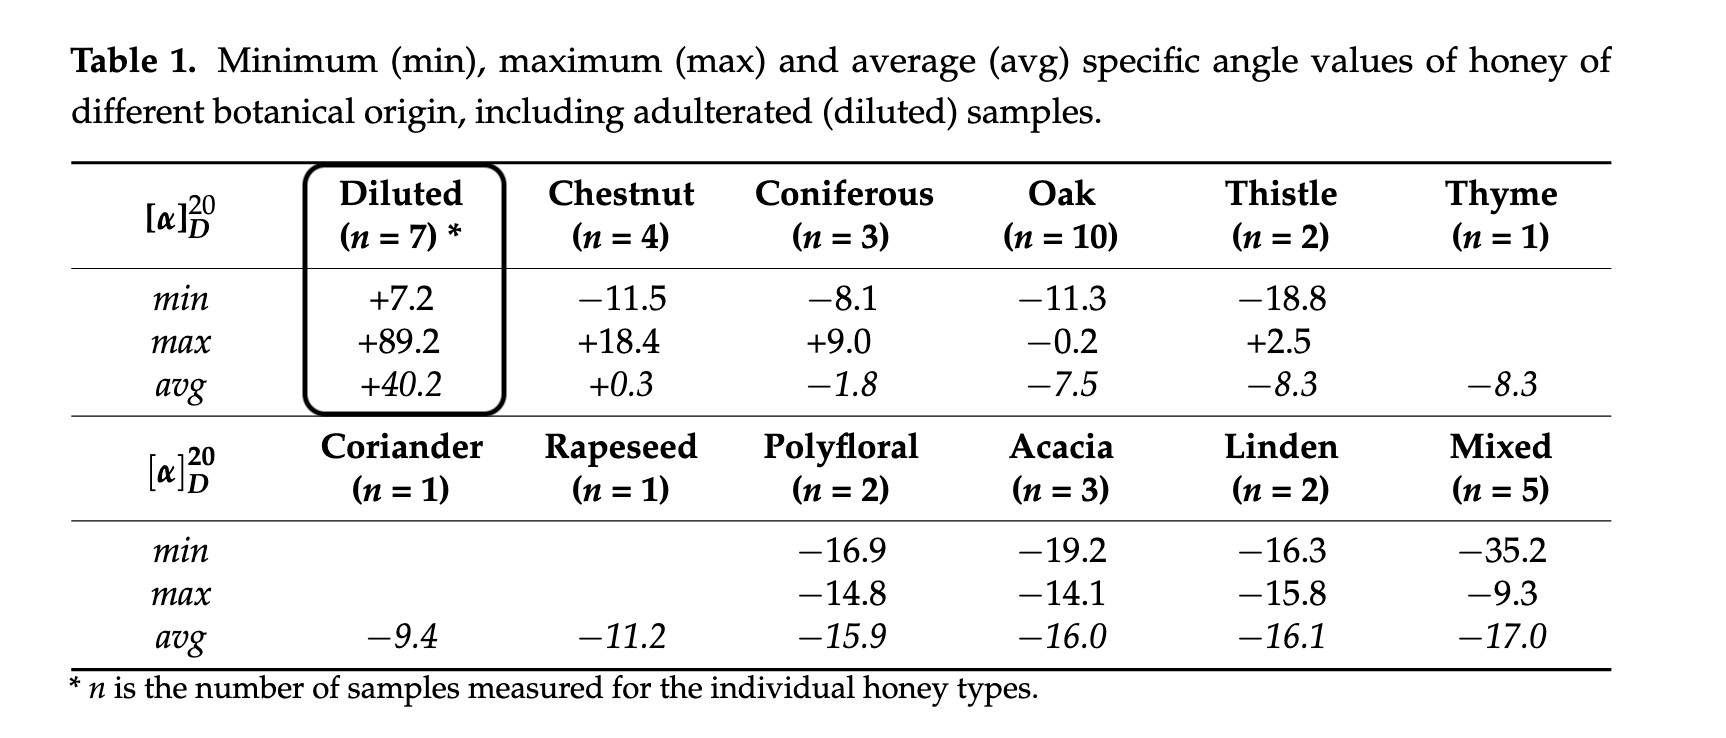
\includegraphics[width=0.7\textwidth]{slike/med2.png}
    \end{center}
\end{frame}

\begin{frame}{Zaključek}
    \begin{itemize}
        \item Optična rotacija saharoze potrjuje teorijo o optični aktivnosti.
        \item Drudejev model dobro opiše odvisnost od valovne dolžine.
        \item Analiza medu: možno razlikovanje naravnega in umetnega medu.
    \end{itemize}
\end{frame}

\begin{frame}{Literatura}
    \footnotesize
    \begin{thebibliography}{9}
        \bibitem{gerginova2022optical}
        D. Gerginova, V. Kurteva, S. Simova,
        \textit{Optical Rotation—A Reliable Parameter for Authentication of Honey?},
        Molecules, 27(24), 8916, 2022.
    \end{thebibliography}
\end{frame}

\end{document}